%% LyX 1.3 created this file.  For more info, see http://www.lyx.org/.
%% Do not edit unless you really know what you are doing.
\documentclass[english, 12pt]{article}
\usepackage{times}
%\usepackage{algorithm2e}
\usepackage{url}
\usepackage{bbm}
\usepackage[T1]{fontenc}
\usepackage[latin1]{inputenc}
\usepackage{geometry}
\geometry{verbose,letterpaper,tmargin=2.5cm,bmargin=2.5cm,lmargin=2.5cm,rmargin=2.5cm}
\usepackage{rotating}
\usepackage{color}
\usepackage{graphicx}
\usepackage{amsmath, amsthm, amssymb}
\usepackage{setspace}
\usepackage{lineno}
\usepackage{hyperref}
\usepackage{bbm}

%\linenumbers
%\doublespacing
%\usepackage[authoryear]{natbib}
\usepackage{natbib} \bibpunct{(}{)}{;}{author-year}{}{,} 

%Pour les rajouts
\usepackage{color}
\definecolor{trustcolor}{rgb}{0,0,1}

\usepackage{dsfont}
\usepackage[warn]{textcomp}
\usepackage{adjustbox}
\usepackage{multirow}
\usepackage{graphicx}
\graphicspath{{../figures/}}
\DeclareMathOperator*{\argmin}{\arg\!\min}

\let\tabbeg\tabular
\let\tabend\endtabular
\renewenvironment{tabular}{\begin{adjustbox}{max width=\textwidth}\tabbeg}{\tabend\end{adjustbox}}

\makeatletter

%%%%%%%%%%%%%%%%%%%%%%%%%%%%%% LyX specific LaTeX commands.
%% Bold symbol macro for standard LaTeX users
%\newcommand{\boldsymbol}[1]{\mbox{\boldmath $#1$}}

%% Because html converters don't know tabularnewline
\providecommand{\tabularnewline}{\\}

\usepackage{babel}
\makeatother


\begin{document}

\section*{Supplementary Material and Methods}

\renewcommand{\thefigure}{S\arabic{figure}}
\setcounter{figure}{0}
\renewcommand{\thetable}{S\arabic{table}}
\setcounter{table}{0}

%%%%%%%%%%%%%%%%%%%%%%%%%%%%%%%%%%%%%%%%%%%%%%%%%%%%%%%%%%%%%%%%%%%%%%%%%%%%%%%%

\subsection*{Model ``COMP''}

For model ``COMP'', we separate the causal SNPs in three equal sets $S_\text{causal}^{(1)}$, $S_\text{causal}^{(2)}$
and $S_\text{causal}^{(3)}$; $S_\text{causal}^{(3)}$ is further separated in two equal sets, $S_\text{causal}^{(3.1)}$ and $S_\text{causal}^{(3.2)}$.
We then compute $$y_i = \underbrace{\sum_{j\in S_\text{causal}^{(1)}} w_j \cdot \widetilde{G_{i,j}}}_\text{linear} + \underbrace{\sum_{j\in S_\text{causal}^{(2)}} w_j \cdot \widetilde{D_{i,j}}}_\text{dominant} + \underbrace{\sum_{\substack{k=1 \\ j_1=e_k^{(3.1)} \\ j_2=e_k^{(3.2)}}}^{k=\left|S_\text{causal}^{(3.1)}\right|} w_{j_1} \cdot \widetilde{G_{i,j_1} G_{i,j_2}}}_\text{interaction} ~~+~~ \epsilon_i~,$$
where $w_j$ are weights generated from a Gaussian or a Laplace distribution, $G_{i,j}$ is the allele count of individual $i$ for SNP $j$, $\widetilde{G_{i,j}}$ corresponds to its standardized version (zero mean and unit variance for all SNPs), $D_{i,j} = \mathds{1}\left\{G_{i,j} \neq 0\right\}$, $\epsilon$ follows a Gaussian distribution $N(0, 1 - h^2)$ and $S_\text{causal}^{(q)}=\left\{e_k^{(q)},~k \in \left\{1, \ldots, \left|S_\text{causal}^{(q)}\right|\right\}\right\}$.
%Note that, because we use the raw genotype counts when coding the interaction terms, the corresponding SNPs also display a marginal effect.

\subsection*{Maximum AUCs} \label{sec:auc-max}

We use three different ways to estimate the maximum achievable AUC for simulations (see supplementary notebook ``oracle'').

First, we use the estimation from equation (3) of \cite{wray2010genetic}. For a prevalence fixed at 30\% and an heritability of 50\% (respectively 80\%), the approximated theoretical values of AUC are 84.1\% (respectively 93.0\%). Note that this approximation is reported to be less accurate for high heritabilities.

Secondly, if we assume that the genetic part of the liabilities follows a Gaussian distribution $N(0, h^2)$ and that the environmental part follows a Gaussian distribution $N(0, 1 - h^2)$, we can estimate the theoretical value of the AUC that can be achieved given the disease heritability $h^2$ (and prevalence $K$) through Monte Carlo simulations. We report AUCs of 84.1\% and 94.1\% for heritabilities of 50\% and 80\%, respectively.

Thirdly, we reproduce the exact same procedure of simulations and, for each combination of parameters (Table 2), we estimate the AUC of the ``oracle'', i.e.\ the true simulated genetic part of the liabilities, through 100 replicates. For every combination of parameters, AUC values of oracles vary between 83.2\% and 84.2\% for an heritability of 50\% and between 93.2\% and 94.1\% for an heritability of 80\%.

Given all these estimates of maximal achievable AUC and for the sake of simplicity, we report maximum AUCs of 84\% (94\%) for heritabilities of 50\% (80\%) whatever are the simulation parameters.


\vspace*{-12pt}

\bibliographystyle{natbib}
\bibliography{refs}


%%%%%%%%%%%%%%%%%%%%%%%%%%%%%%%%%%%%%%%%%%%%%%%%%%%%%%%%%%%%%%%%%%%%%%%%%%%%%%%%

\newpage

\begin{table}[ht]
\centering
\begin{tabular}{|l|cccc|r|}
\hline
Population & UK & Finland & Netherlands & Italy & Total\\
\hline
Cases & 2569 & 637 & 795 & 495 & 4496\\
Controls & 7492 & 1799 & 828 & 540 & 10659\\
\hline
Total & 10061 & 2436 & 1623 & 1035 & 15155\\
\hline
\end{tabular}
\caption{Number of individuals by population and disease status in the celiac disease case-control study (after quality control, genotyped on 281,122 SNPs).\label{tab:celiac-data}}
\end{table}

%%%%%%%%%%%%%%%%%%%%%%%%%%%%%%%%%%%%%%%%%%%%%%%%%%%%%%%%%%%%%%%%%%%%%%%%%%%%%%%%

% latex table generated in R 3.4.1 by xtable 1.8-2 package
% Thu Oct 26 16:46:26 2017
\begin{table}[ht]
\centering
\begin{tabular}{ccccccccccccccc}
  \hline
1.00e+00 & 7.22e-01 & 5.87e-01 & 4.20e-01 & 2.43e-01 & 1.00e-01 & 2.35e-02 & 2.21e-03 & 4.69e-05 & 8.81e-08 & 3.18e-12 & 1.83e-19 & 2.89e-31 & 1.70e-50 & 7.71e-82 \\ 
  5.00e-08 & 7.05e-01 & 5.65e-01 & 3.95e-01 & 2.20e-01 & 8.47e-02 & 1.79e-02 & 1.42e-03 & 2.28e-05 & 2.73e-08 & 4.69e-13 & 8.08e-21 & 1.80e-33 & 4.30e-54 & 1.06e-87 \\ 
  7.94e-01 & 6.87e-01 & 5.42e-01 & 3.69e-01 & 1.97e-01 & 7.08e-02 & 1.34e-02 & 8.83e-04 & 1.05e-05 & 7.74e-09 & 6.03e-14 & 2.86e-22 & 7.73e-36 & 5.97e-58 & 5.49e-94 \\ 
  7.81e-01 & 6.69e-01 & 5.19e-01 & 3.43e-01 & 1.75e-01 & 5.85e-02 & 9.79e-03 & 5.31e-04 & 4.61e-06 & 2.01e-09 & 6.69e-15 & 7.92e-24 & 2.24e-38 & 4.37e-62 & 1.00e-100 \\ 
  7.67e-01 & 6.50e-01 & 4.95e-01 & 3.18e-01 & 1.54e-01 & 4.76e-02 & 7.01e-03 & 3.08e-04 & 1.90e-06 & 4.72e-10 & 6.32e-16 & 1.70e-25 & 4.26e-41 & 1.61e-66 &  \\ 
  7.53e-01 & 6.30e-01 & 4.70e-01 & 2.93e-01 & 1.35e-01 & 3.82e-02 & 4.90e-03 & 1.72e-04 & 7.31e-07 & 1.00e-10 & 5.04e-17 & 2.75e-27 & 5.16e-44 & 2.83e-71 &  \\ 
  7.38e-01 & 6.09e-01 & 4.46e-01 & 2.68e-01 & 1.17e-01 & 3.02e-02 & 3.33e-03 & 9.18e-05 & 2.63e-07 & 1.89e-11 & 3.35e-18 & 3.31e-29 & 3.84e-47 & 2.26e-76 &  \\ 
   \hline
\end{tabular}
\caption{The 102 thresholds used for the C+T method for this study.\label{tab:thr}}
\end{table}

%%%%%%%%%%%%%%%%%%%%%%%%%%%%%%%%%%%%%%%%%%%%%%%%%%%%%%%%%%%%%%%%%%%%%%%%%%%%%%%%

\newpage
\begin{figure}[h]
\centerline{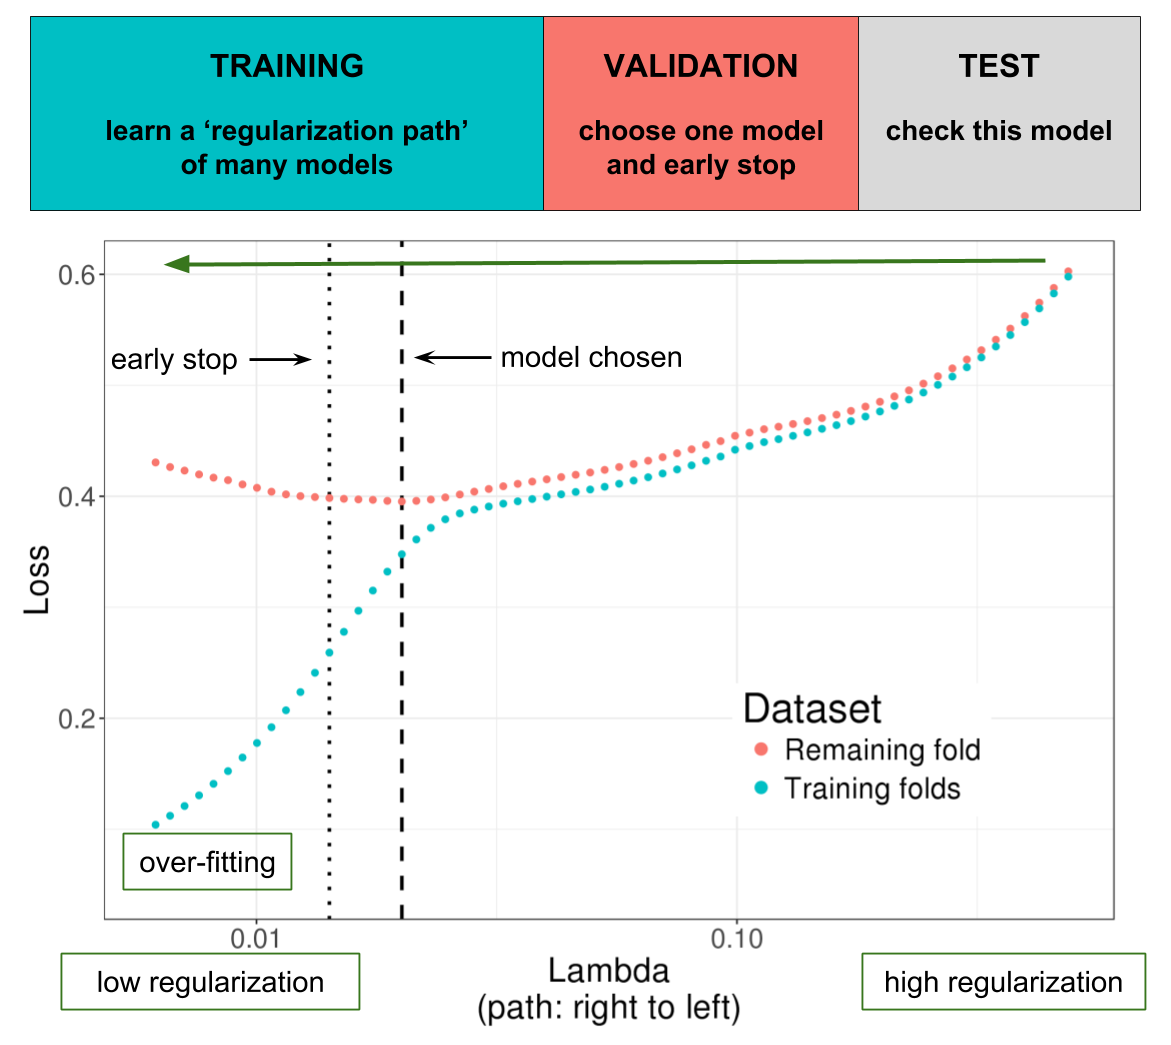
\includegraphics[width=\textwidth]{simple-CMSA}}
\caption{Illustration of one turn of the Cross-Model Selection and Averaging (CMSA) procedure. First, this procedure separates the training set in $K$ folds (e.g.\ 10 folds). 
Secondly, in turn, each fold is considered as an inner validation set (red) and the other ($K - 1$) folds form an inner training set (blue). A ``regularization path'' of models is trained on the inner training set and the corresponding predictions (scores) for the inner validation set are computed. The model that minimizes the loss on the inner validation set is selected. Finally, the $K$ resulting models are averaged. 
We also use this procedure to derive an early stopping criterion so that the algorithm does not need to evaluate the whole regularization paths, making this procedure much faster.}
\label{fig:CMSA}
\end{figure}

%%%%%%%%%%%%%%%%%%%%%%%%%%%%%%%%%%%%%%%%%%%%%%%%%%%%%%%%%%%%%%%%%%%%%%%%%%%%%%%%

\newpage
\begin{figure}[h]
\centerline{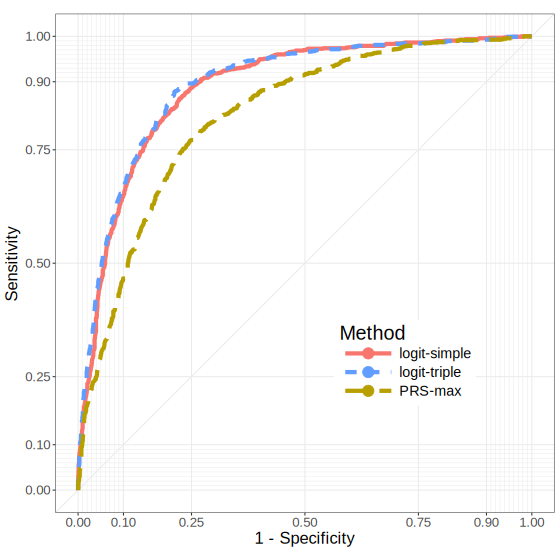
\includegraphics[width=\textwidth]{celiac-roc}}
\caption{ROC Curves for C+T-max, PLR and PLR3 for the celiac disease dataset. Models were trained using 12,000 individuals. These are results projecting these models on the remaining 3155 individuals. The figure is plotted using R package plotROC \cite[]{sachs2017plotroc}.\label{fig:celiac-roc}}
\end{figure}

%%%%%%%%%%%%%%%%%%%%%%%%%%%%%%%%%%%%%%%%%%%%%%%%%%%%%%%%%%%%%%%%%%%%%%%%%%%%%%%%

\newpage
\begin{figure}[h]
\centerline{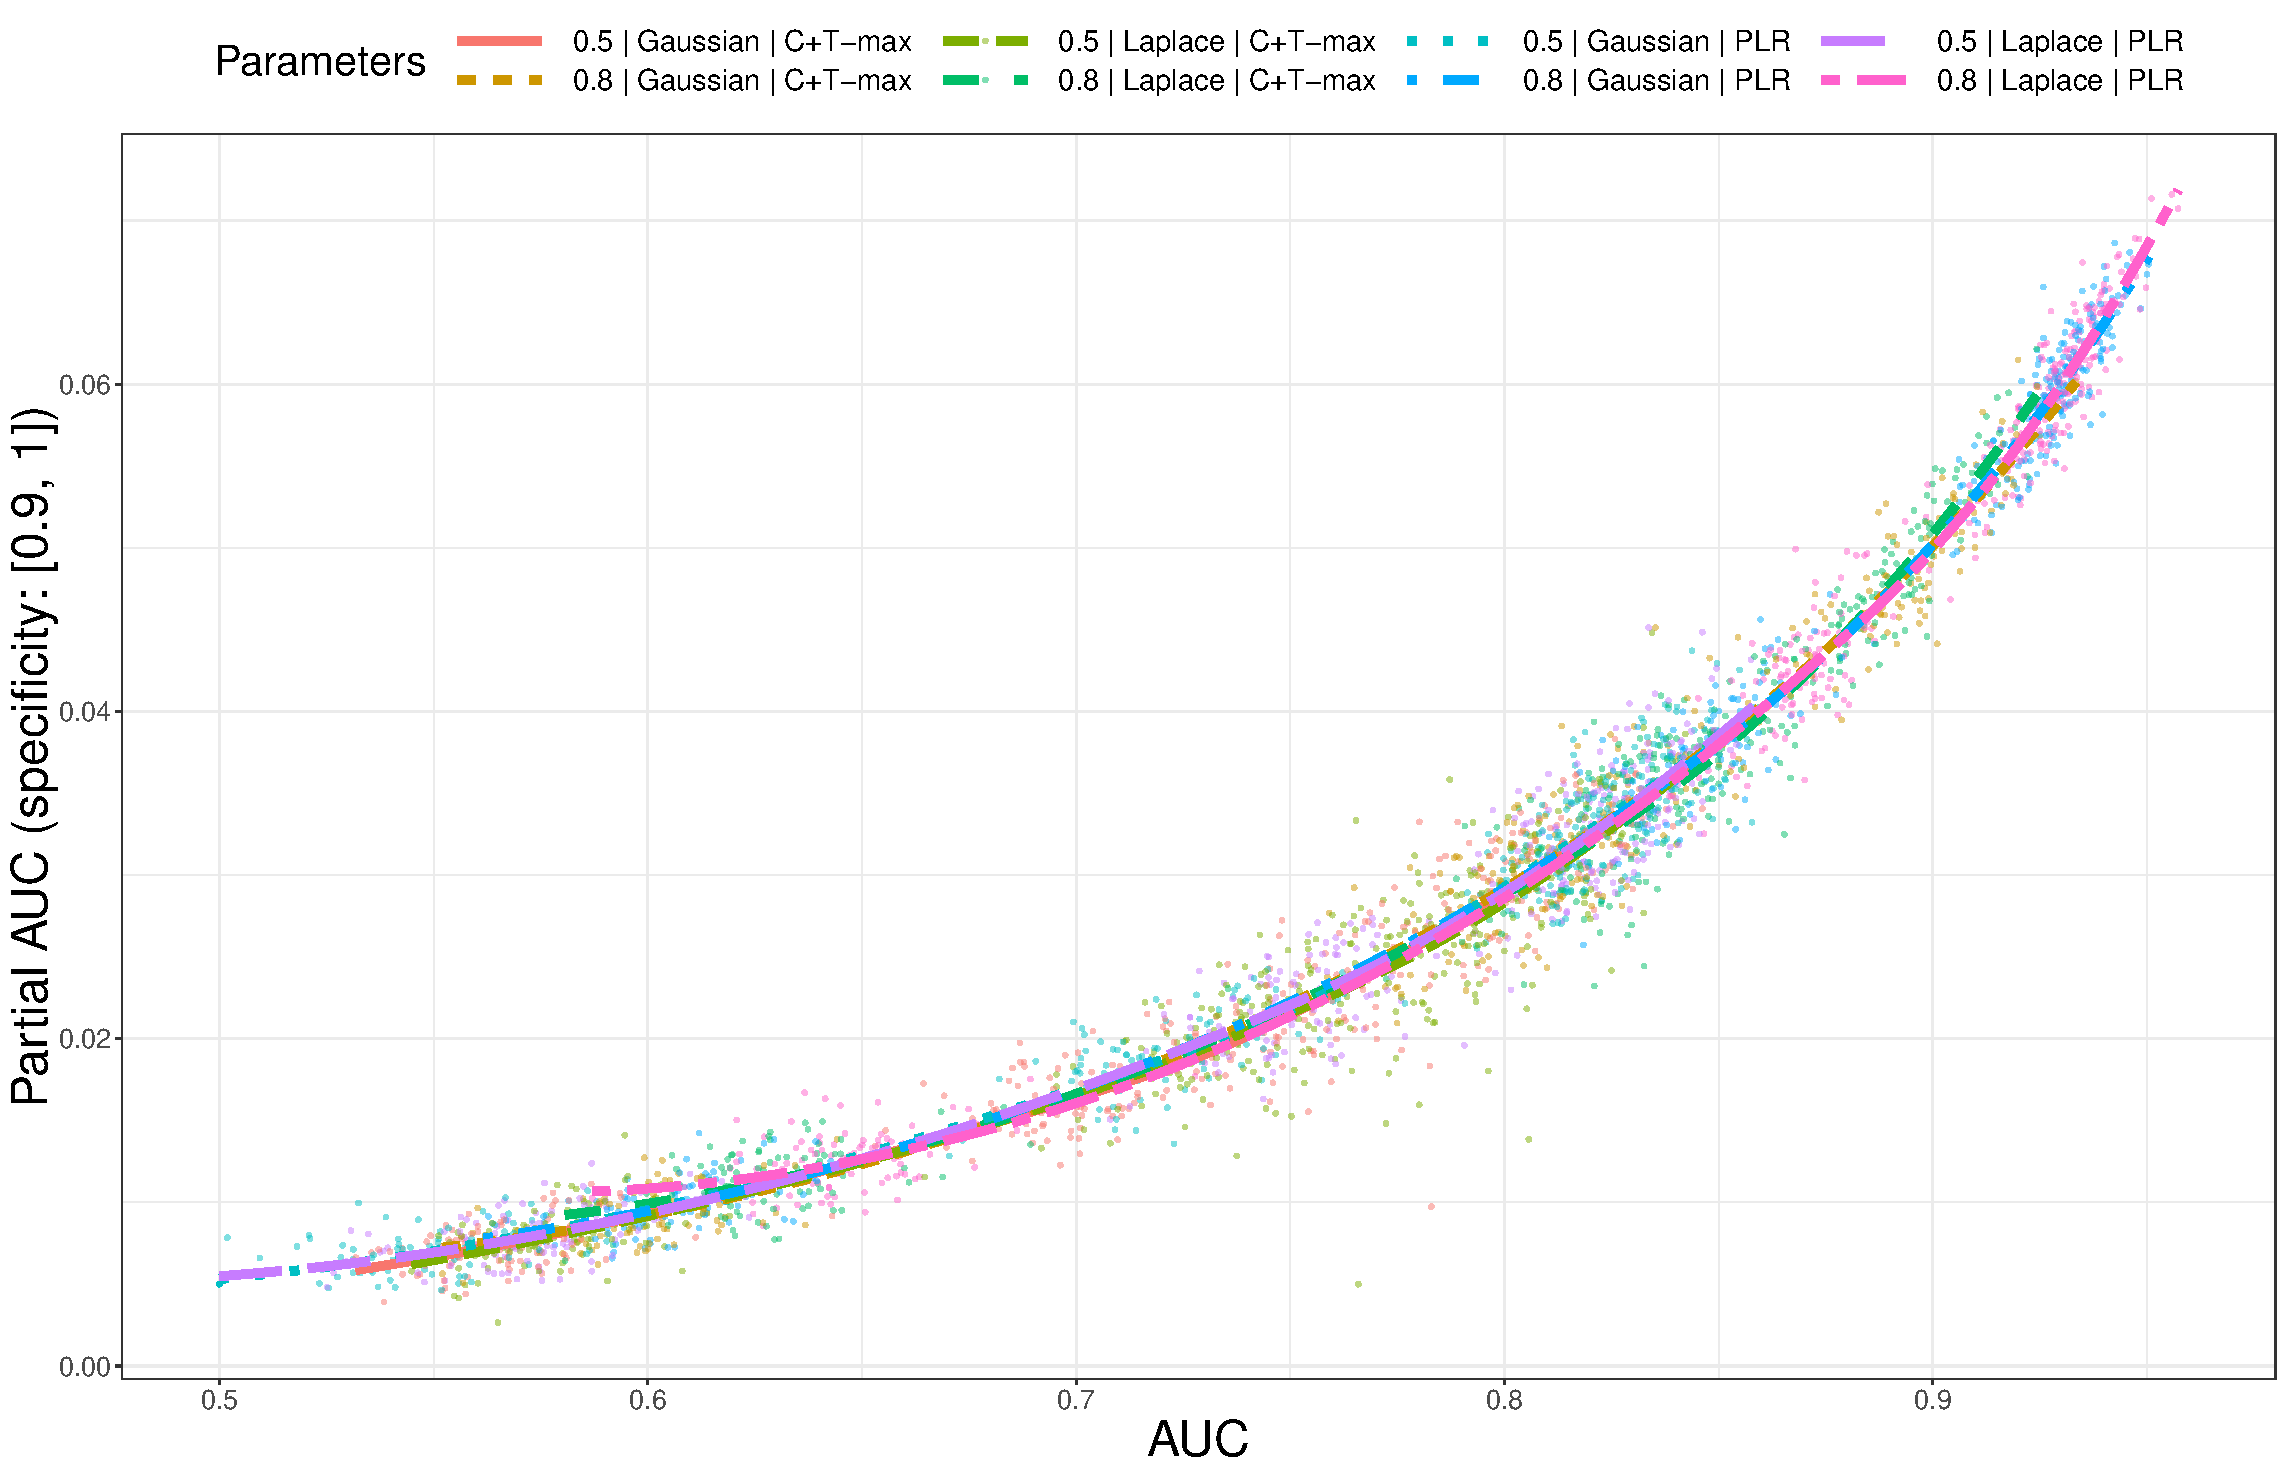
\includegraphics[width=\textwidth]{supp-AUC-corr}}
\caption{Correlation between AUC and partial AUC values in scenario \textnumero1. There is a Spearman correlation of 98\% between values of AUC and partial AUC. The relation between the two values are the same whatever are the disease heritability, distribution of effects and method used.\label{fig:supp-AUC-corr}}
\end{figure}

%%%%%%%%%%%%%%%%%%%%%%%%%%%%%%%%%%%%%%%%%%%%%%%%%%%%%%%%%%%%%%%%%%%%%%%%%%%%%%%%

\newpage
\begin{figure}[h]
\centerline{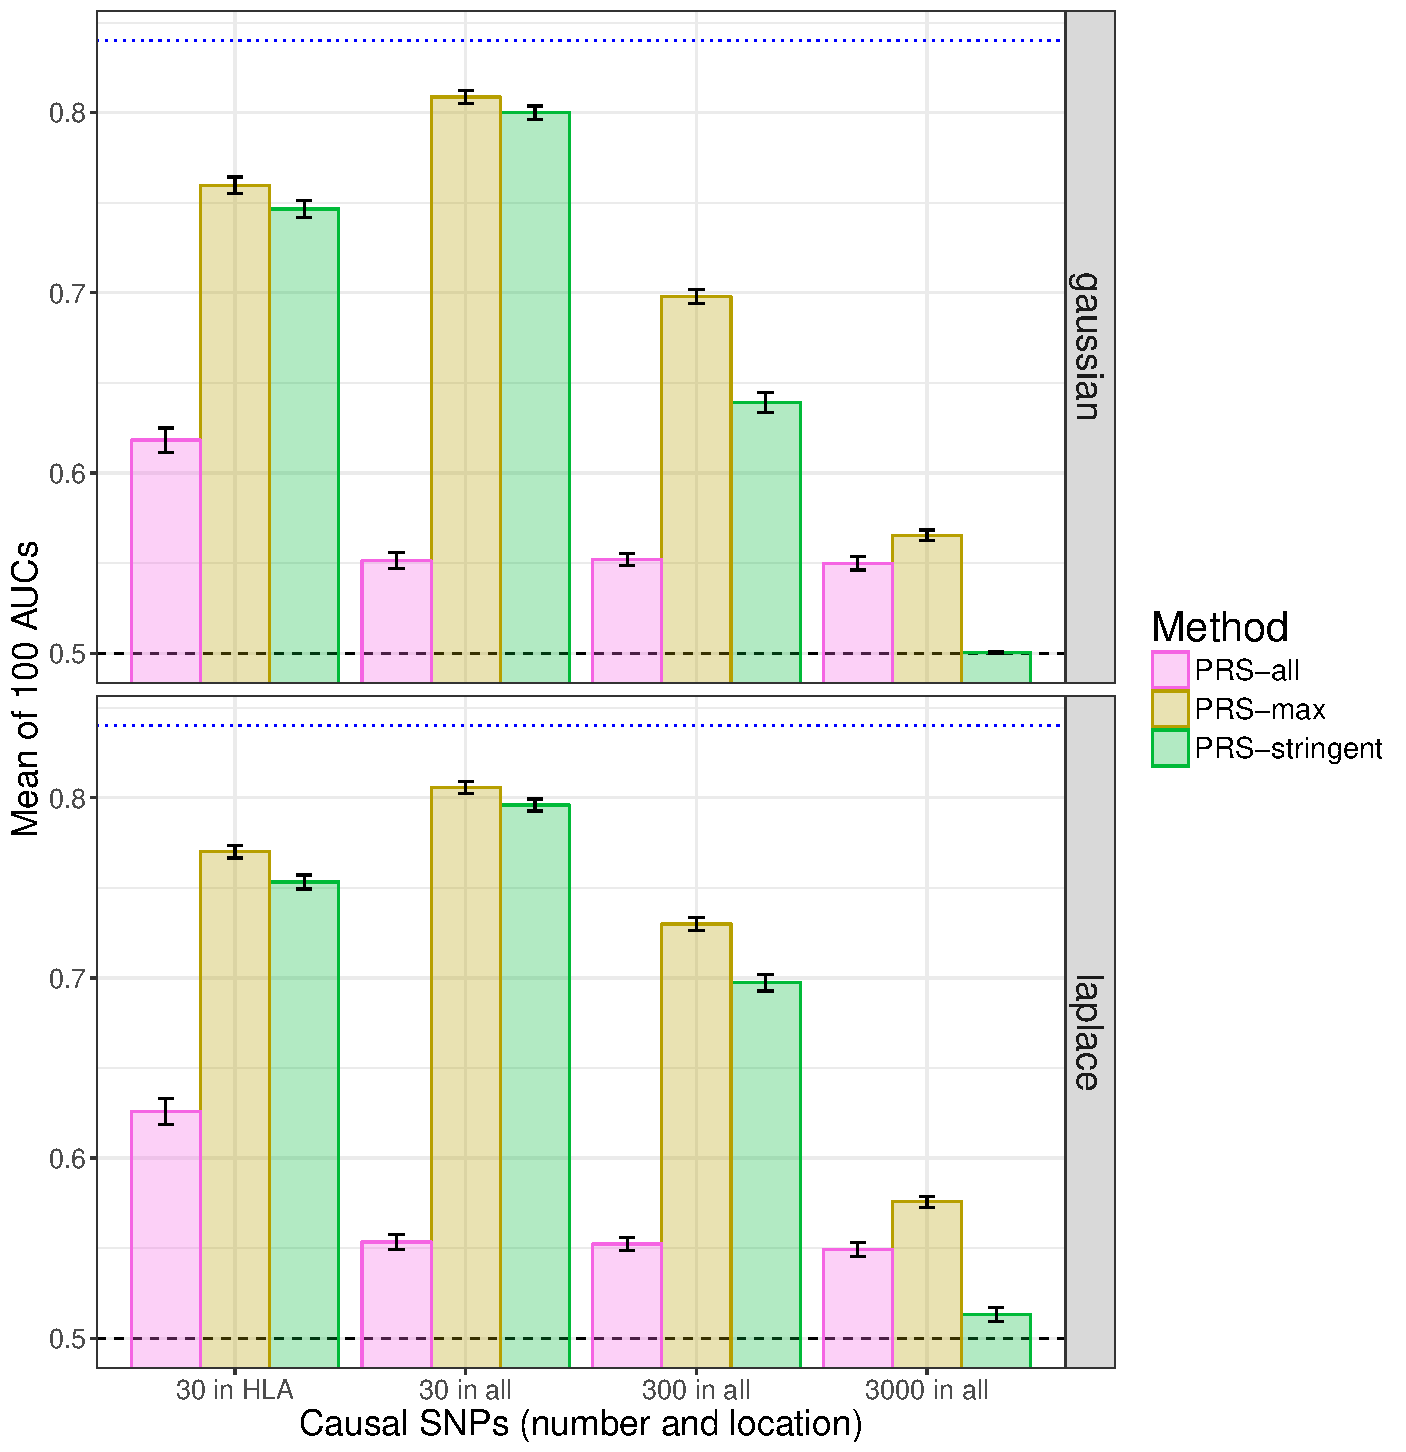
\includegraphics[width=\textwidth]{supp-AUC-PRS}}
\caption{Comparison of three different p-value thresholds used in the C+T method in scenario \textnumero1 for model ``ADD''. Mean AUC over 100 simulations. Upper (lower) panels are presenting results for effets following a Gaussian (Laplace) distribution and left (right) panels are presenting results for an heritability of 0.5 (0.8). Error bars are representing $\pm 2 \text{SD}$ of $10^5$ non-parametric bootstrap of the mean AUC. The blue dotted line represents the maximum achievable AUC.}
\label{fig:supp-AUC-PRS}
\end{figure}

%%%%%%%%%%%%%%%%%%%%%%%%%%%%%%%%%%%%%%%%%%%%%%%%%%%%%%%%%%%%%%%%%%%%%%%%%%%%%%%%

\newpage
\begin{figure}[h]
\centerline{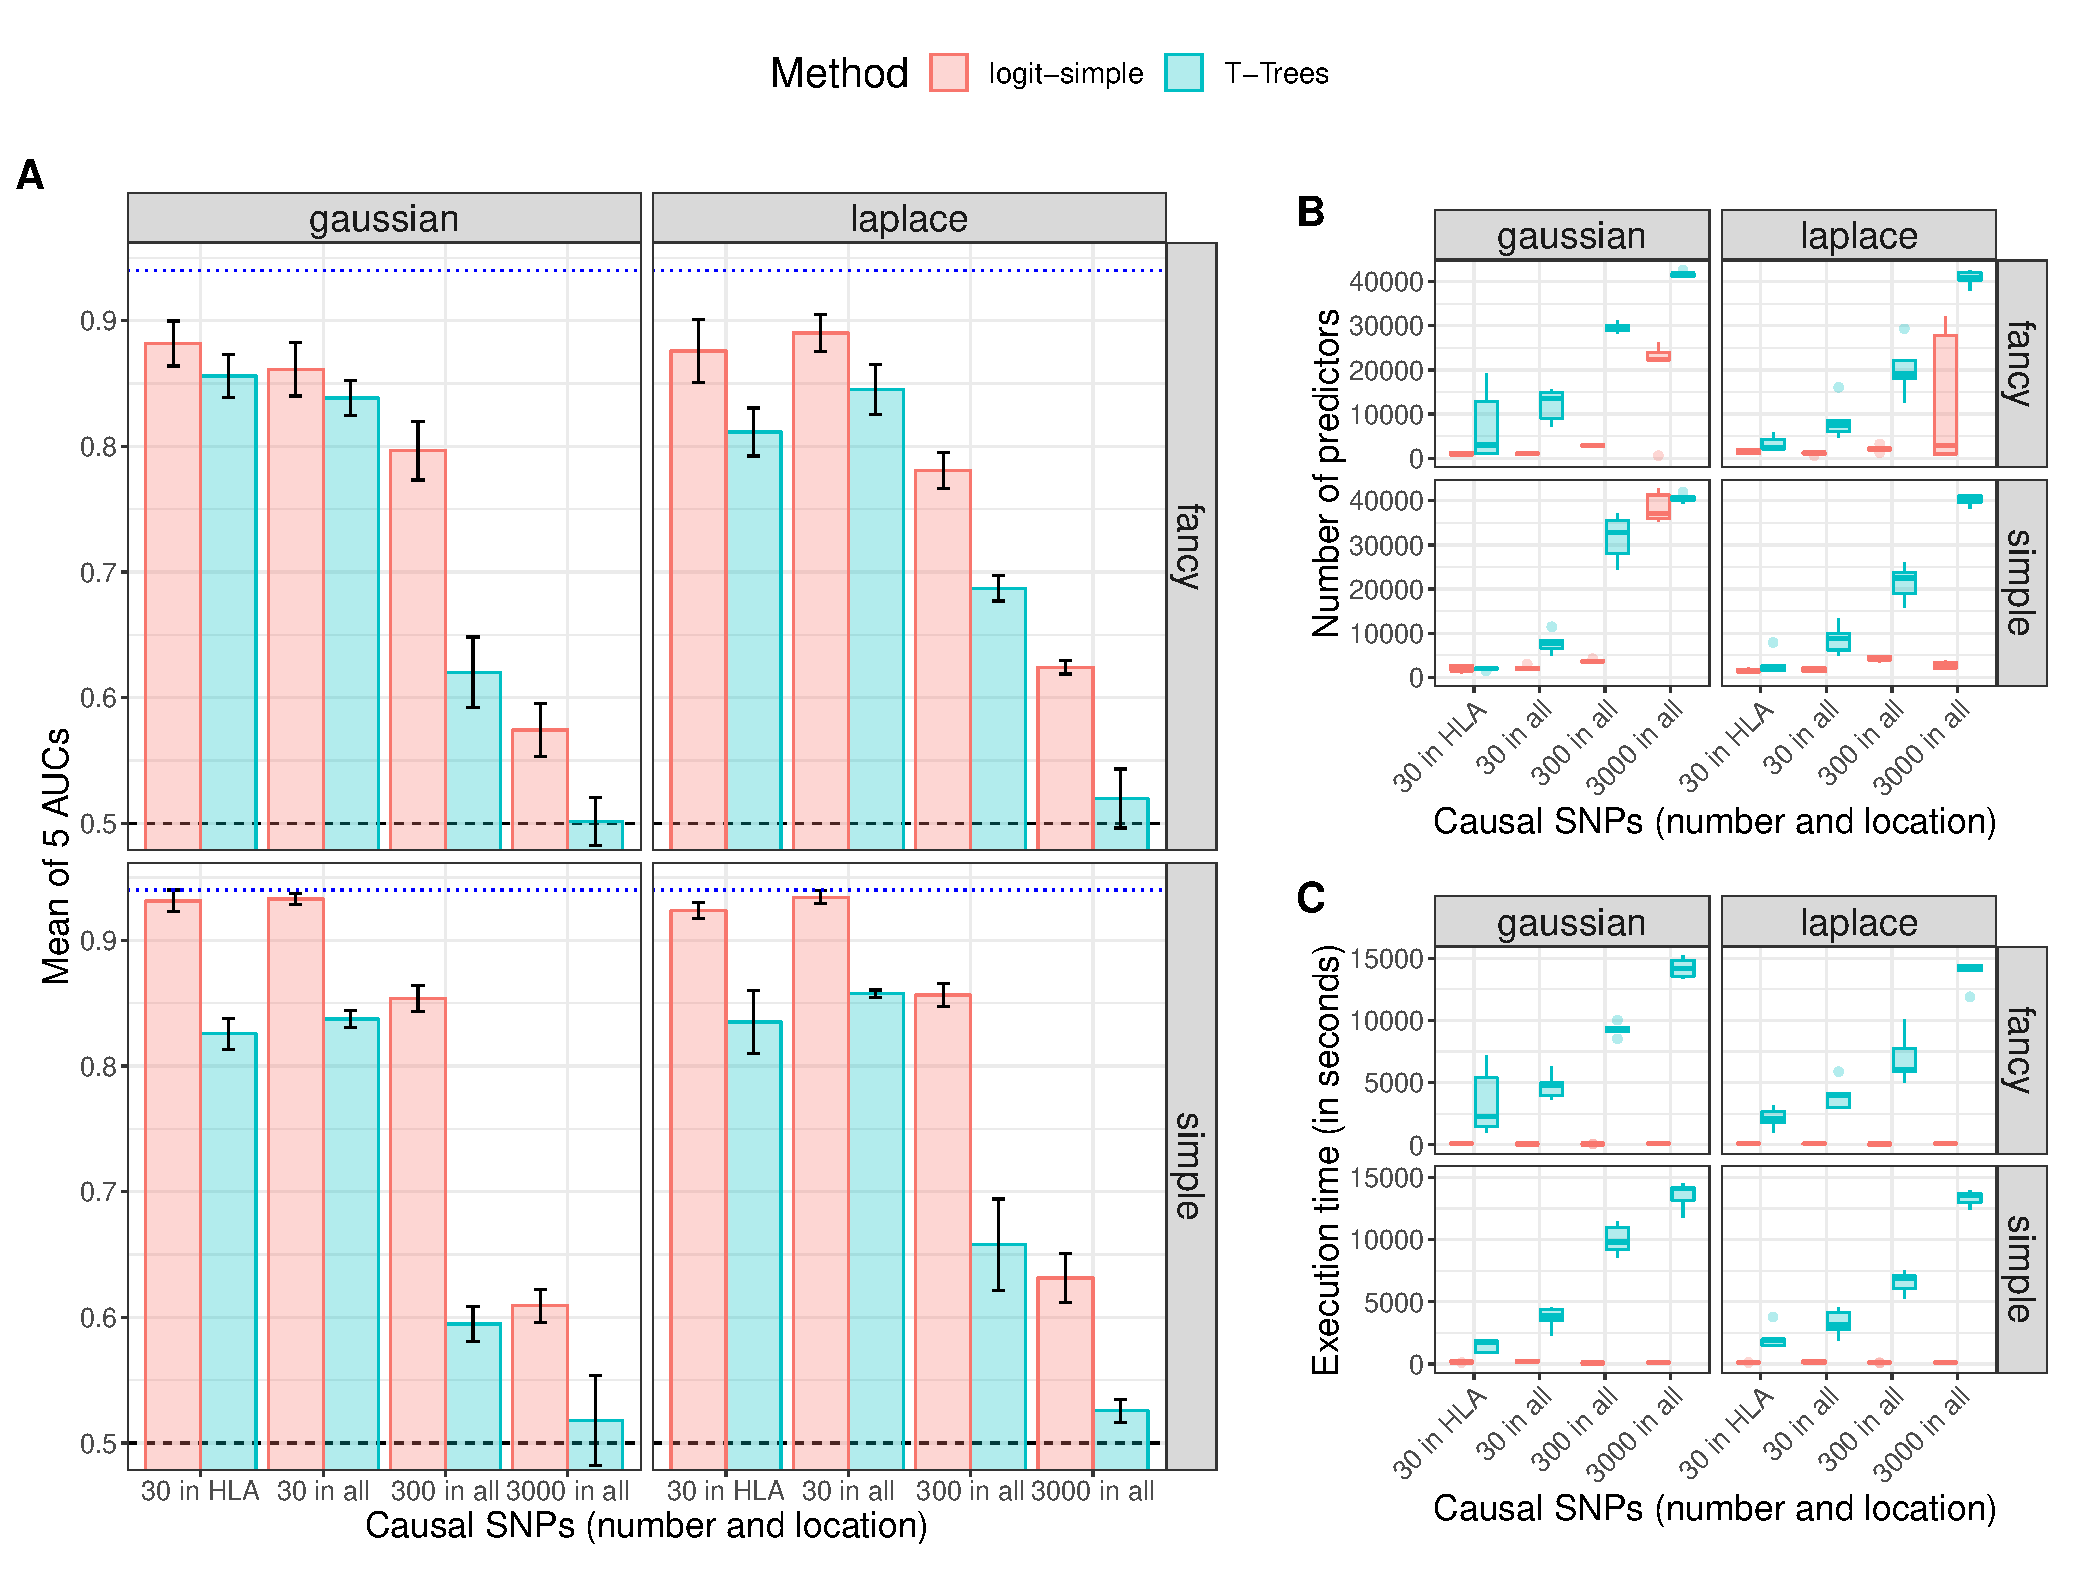
\includegraphics[width=\textwidth]{supp-ttrees}}
\caption{Comparison of T-Trees and PLR in scenario \textnumero1 for an heritability of 80\%. Vertical panels are presenting results for effects following a Gaussian or Laplace distribution. Horizontal panels are presenting results for models ``ADD'' and ``COMP'' for simulating phenotypes. \textbf{A:} Mean AUC over 5 simulations. Error bars are representing $\pm 2 \text{SD}$ of $10^5$ non-parametric bootstrap of the mean AUC. The blue dotted line represents the maximum achievable AUC. \textbf{B:} Boxplots of numbers of predictors used by the methods for 5 simulations. \textbf{C:} Boxplots of execution times for 5 simulations.}
\label{fig:supp-ttrees}
\end{figure}

%%%%%%%%%%%%%%%%%%%%%%%%%%%%%%%%%%%%%%%%%%%%%%%%%%%%%%%%%%%%%%%%%%%%%%%%%%%%%%%%

\newpage
\begin{figure}[h]
\centerline{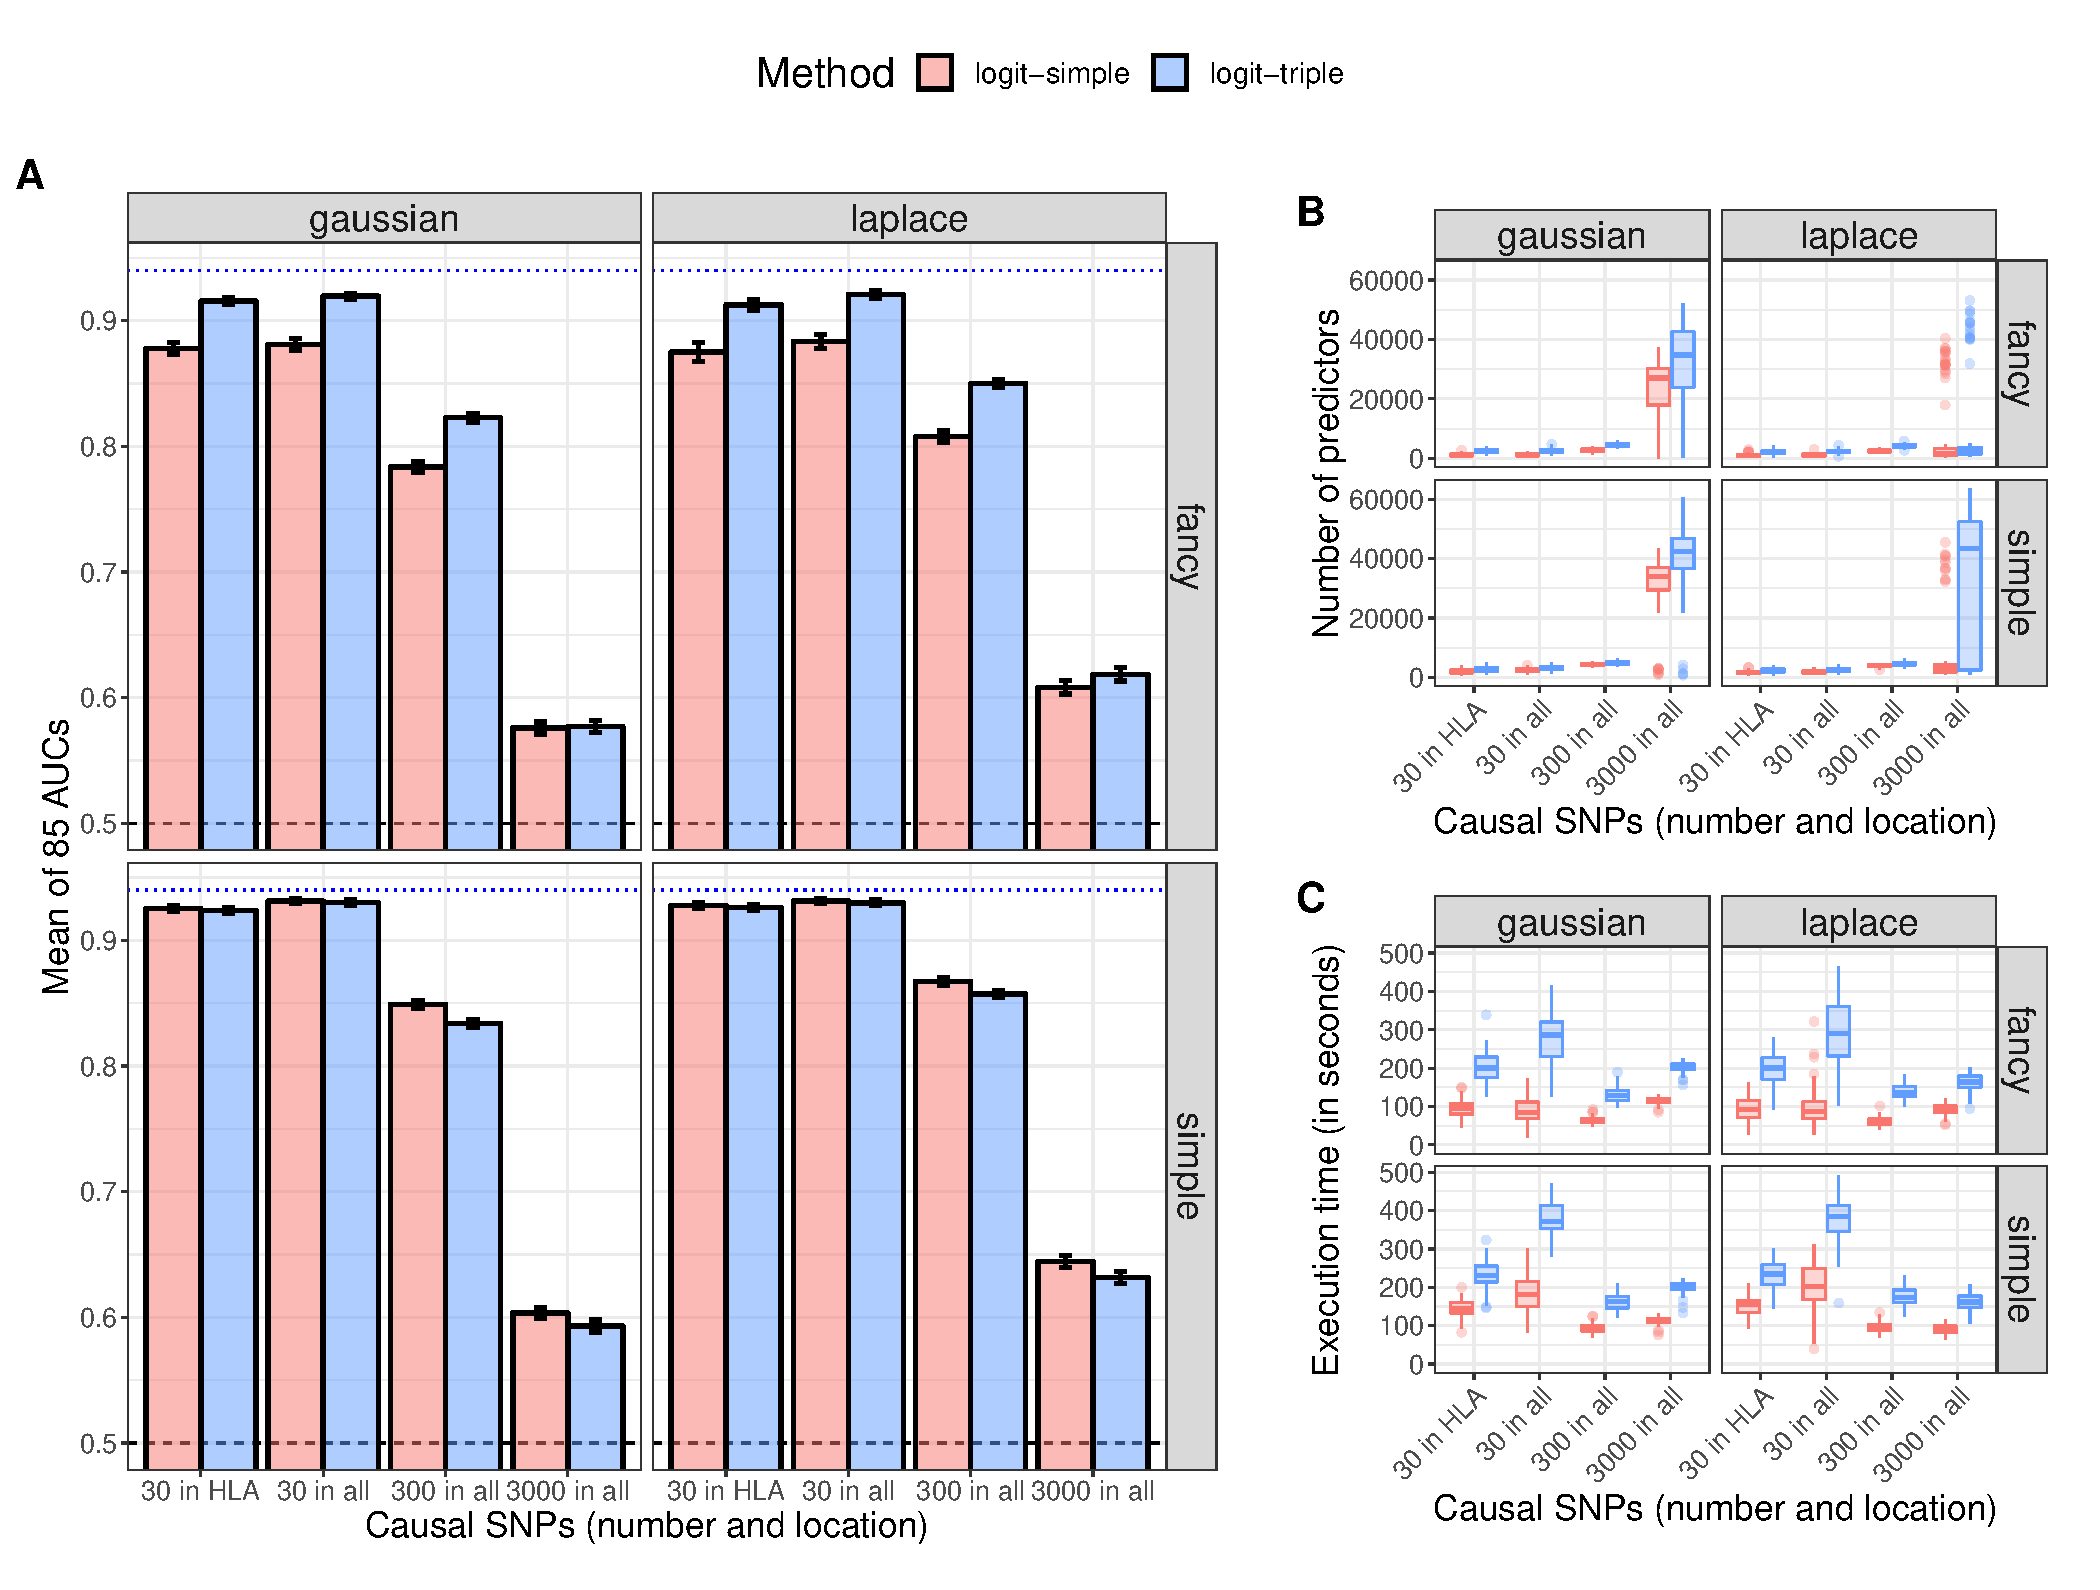
\includegraphics[width=\textwidth]{supp-triple}}
\caption{Comparison of PLR3 and PLR in scenario \textnumero1 for an heritability of 80\%. Vertical panels are presenting results for effects following a Gaussian or Laplace distribution. Horizontal panels are presenting results for models ``ADD'' and ``COMP'' for simulating phenotypes. \textbf{A:} Mean AUC over 100 simulations. Error bars are representing $\pm 2 \text{SD}$ of $10^5$ non-parametric bootstrap of the mean AUC. The blue dotted line represents the maximum achievable AUC. \textbf{B:} Boxplots of numbers of predictors used by the methods for 100 simulations. \textbf{C:} Boxplots of execution times for 100 simulations.}
\label{fig:supp-triple}
\end{figure}


\newpage
\begin{figure}[h]
\centerline{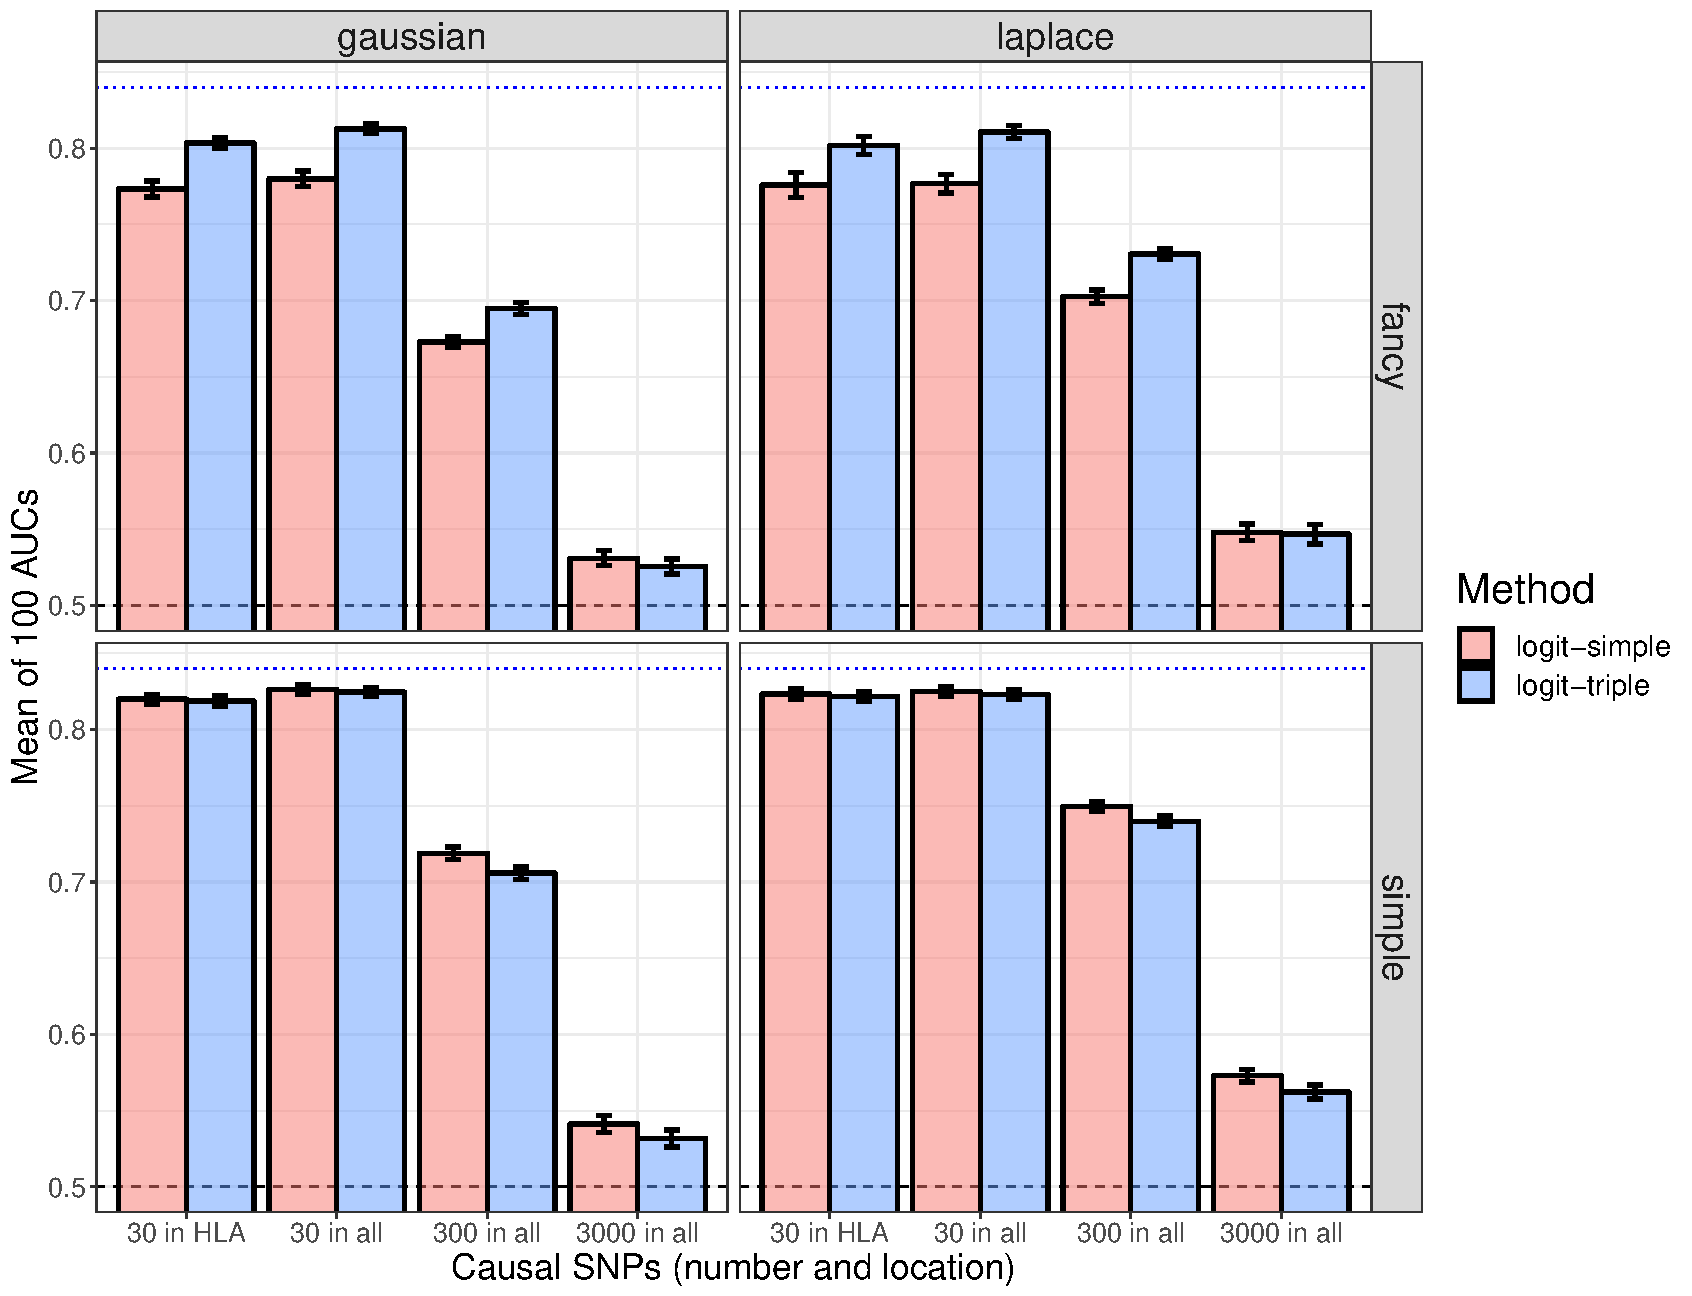
\includegraphics[width=\textwidth]{supp-AUC-triple}}
\caption{Comparison of PLR3 and PLR in scenario \textnumero1 for an heritability of 50\%. Vertical panels are presenting results for effects following a Gaussian or Laplace distribution. Horizontal panels are presenting results for models ``ADD'' and ``COMP'' for simulating phenotypes. \textbf{A:} Mean AUC over 100 simulations. Error bars are representing $\pm 2 \text{SD}$ of $10^5$ non-parametric bootstrap of the mean AUC. The blue dotted line represents the maximum achievable AUC.}
\label{fig:supp-AUC-triple}
\end{figure}

%%%%%%%%%%%%%%%%%%%%%%%%%%%%%%%%%%%%%%%%%%%%%%%%%%%%%%%%%%%%%%%%%%%%%%%%%%%%%%%%

\newpage
\begin{figure}[h]
\centerline{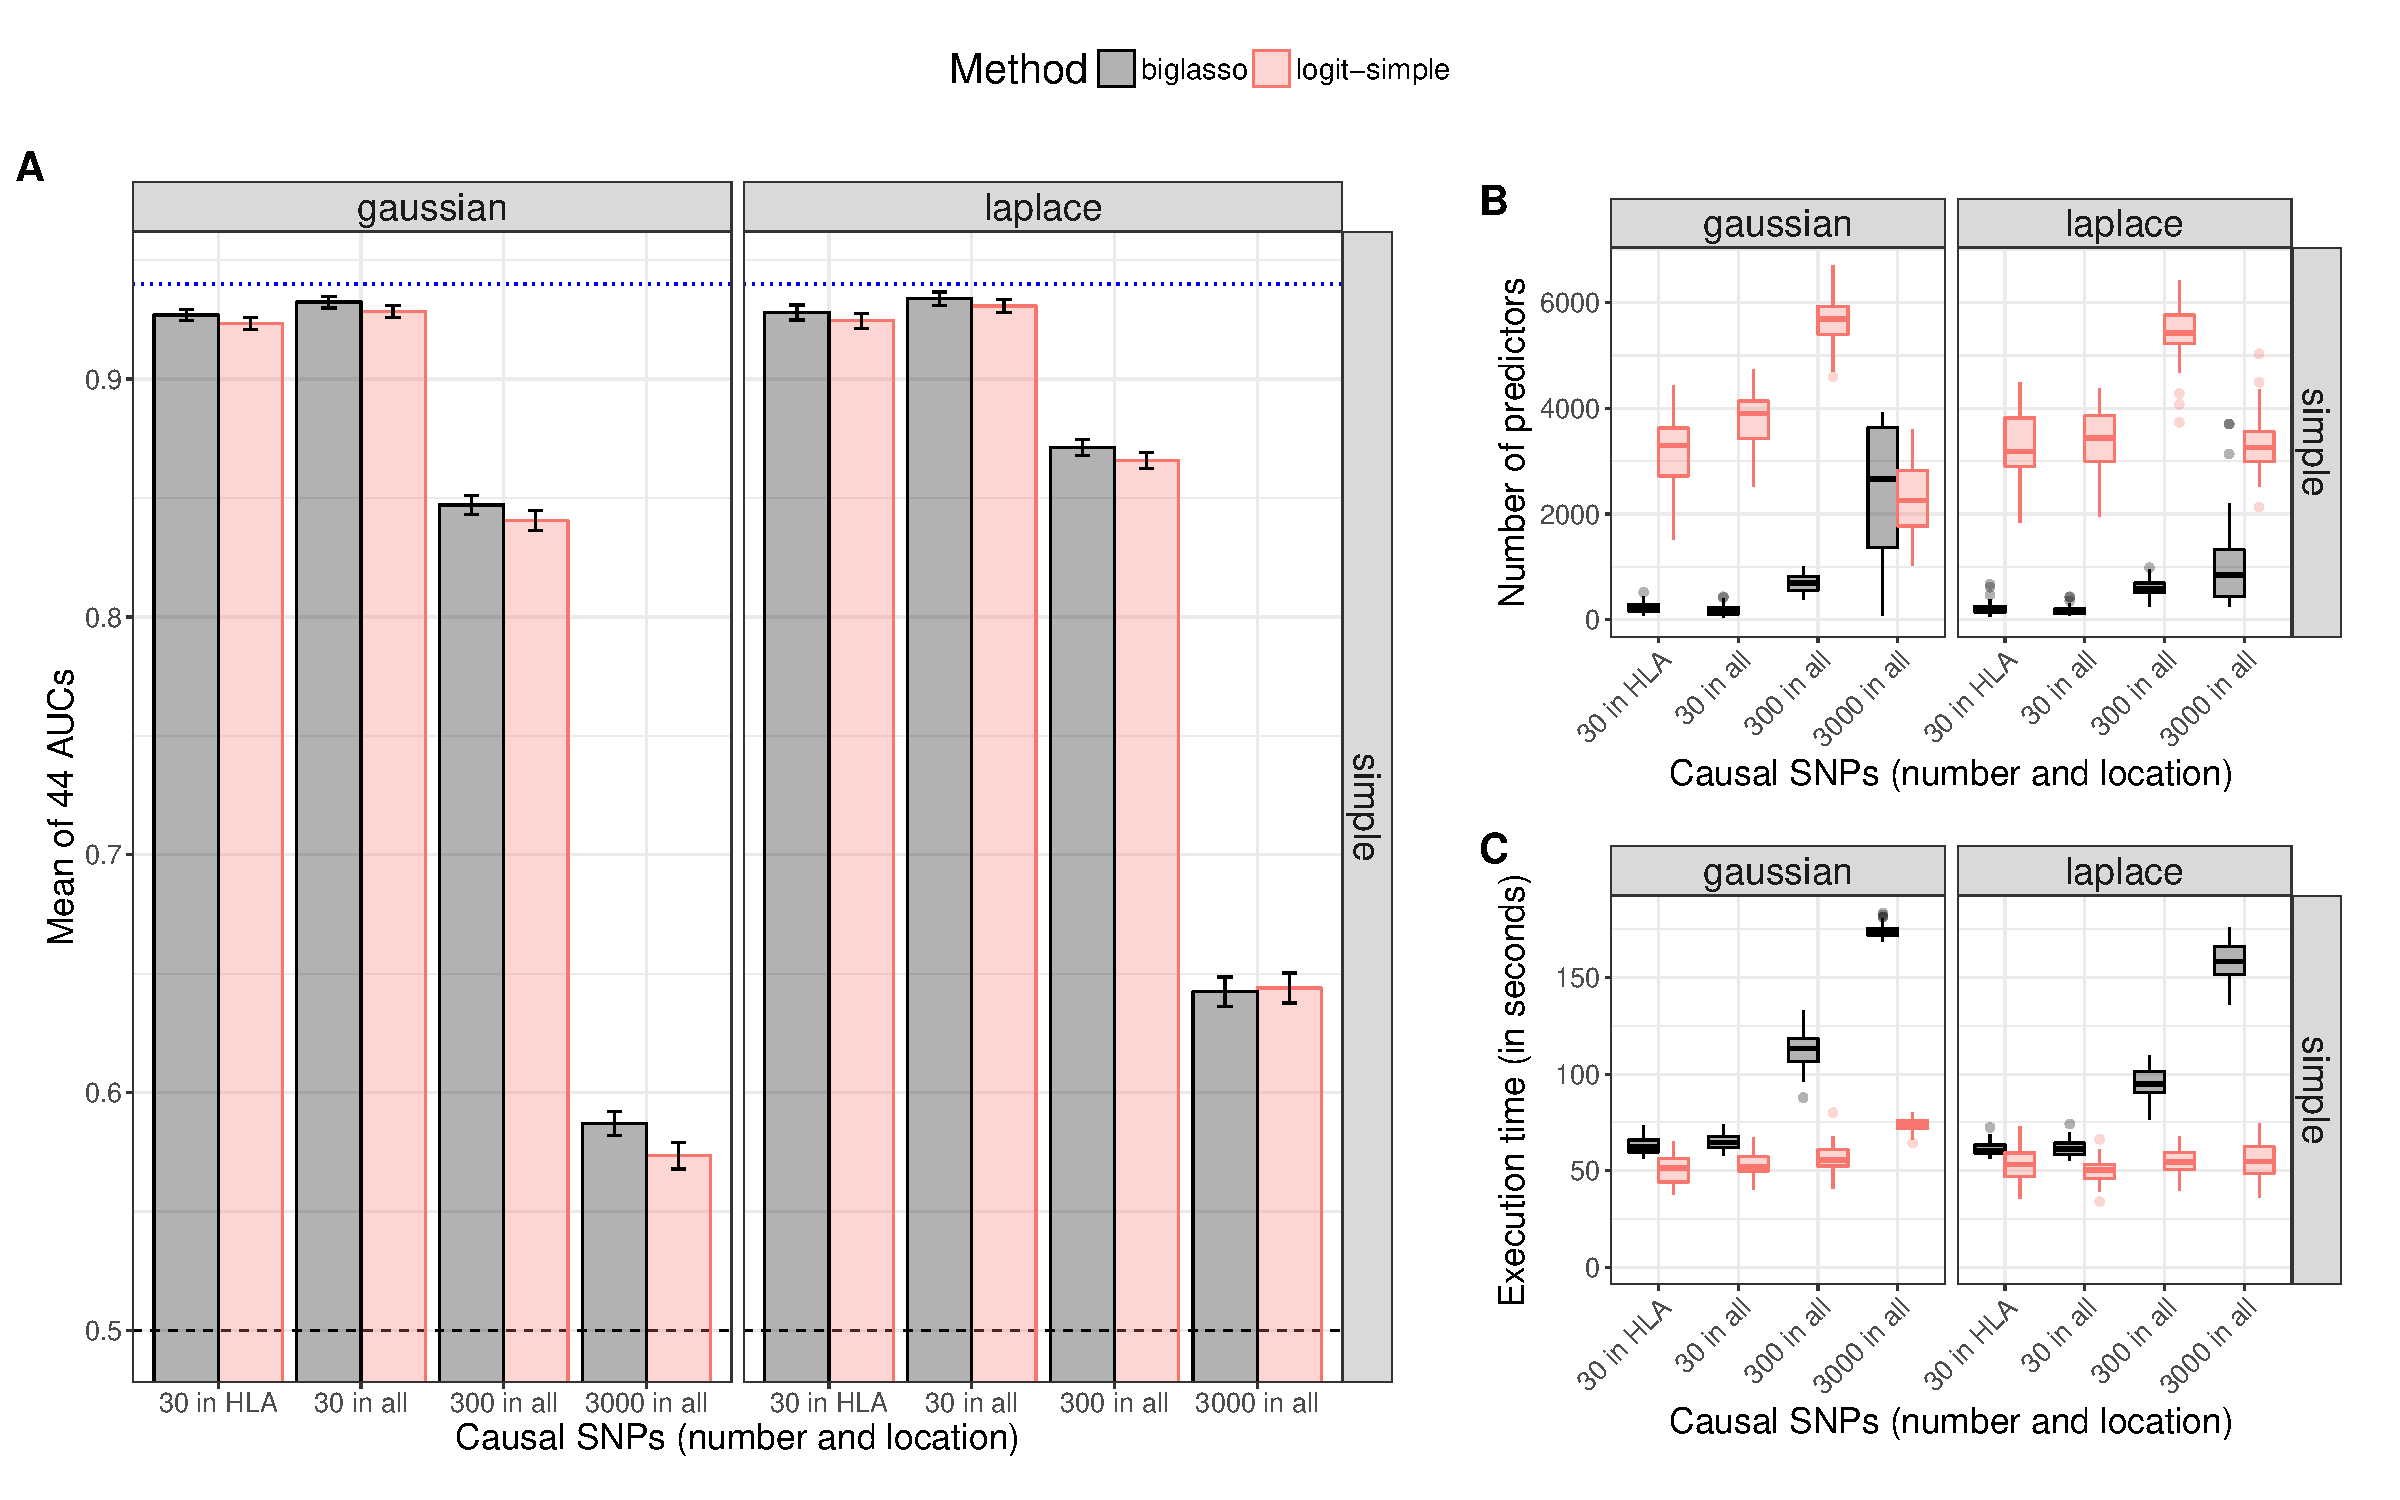
\includegraphics[width=\textwidth]{supp-biglasso}}
\caption{Comparison of PLR and the best prediction (among 100 tested $\lambda$ values) for ``biglasso'' (another implementation of penalized logistic regression -- \cite{zeng2017efficient}) in scenario \textnumero1. Simulations use model ``ADD'', an heritability of 80\% and $\alpha = 1$. Vertical panels are presenting results for effects following a Gaussian or Laplace distribution. \textbf{A:} Mean AUC over 100 simulations. Error bars are representing $\pm 2 \text{SD}$ of $10^5$ non-parametric bootstrap of the mean AUC. The blue dotted line represents the maximum achievable AUC. \textbf{B:} Boxplots of numbers of predictors used by the methods for 100 simulations. \textbf{C:} Boxplots of execution times for 100 simulations.}
\label{fig:supp-biglasso}
\end{figure}

%%%%%%%%%%%%%%%%%%%%%%%%%%%%%%%%%%%%%%%%%%%%%%%%%%%%%%%%%%%%%%%%%%%%%%%%%%%%%%%%

\newpage
\begin{figure}[h]
\centerline{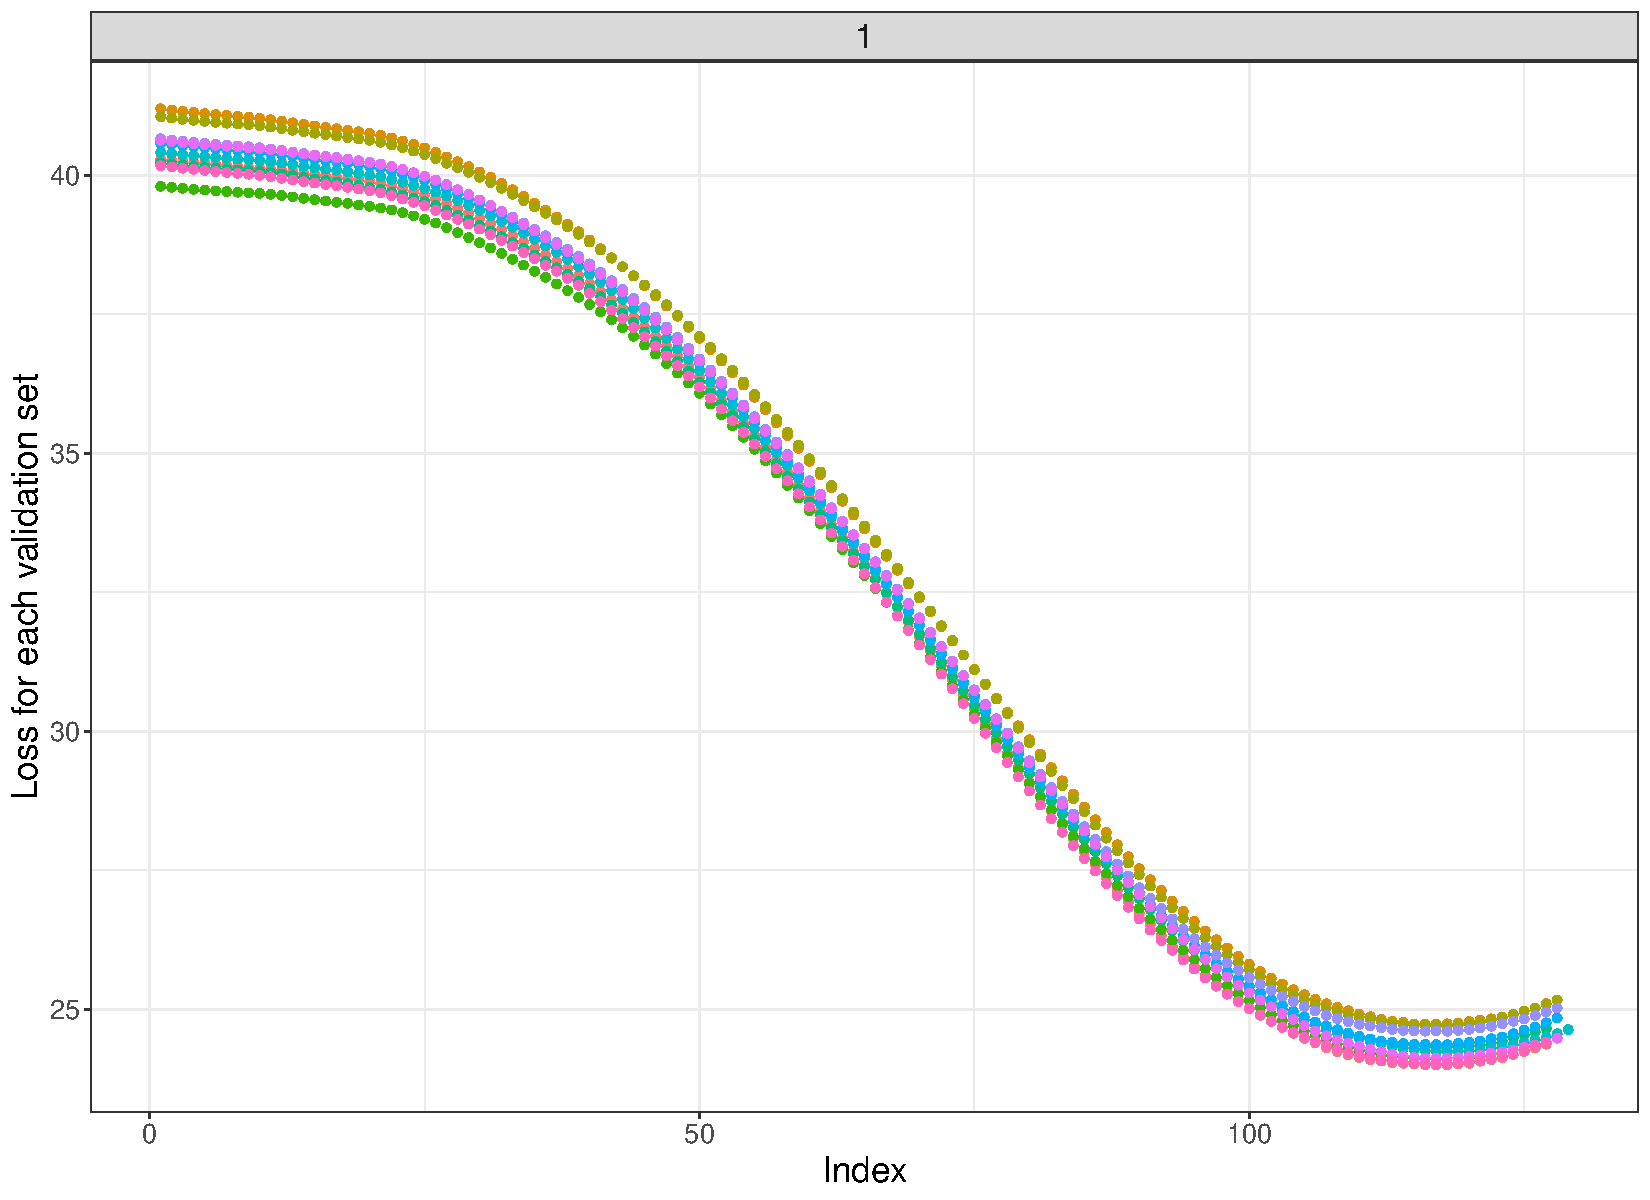
\includegraphics[width=\textwidth]{supp-lasso-path-height}}
\caption{Regularization path for `K = 10' validation sets when fitting our L1-penalized linear regression on 350,000 individuals of the UK Biobank. This plot can be obtained by using the `plot()' method on the object resulting from this fitting. This fitting used `nlambda = 200` and `n.abort = 10' (the defaults).}
\label{fig:supp-path}
\end{figure}

%%%%%%%%%%%%%%%%%%%%%%%%%%%%%%%%%%%%%%%%%%%%%%%%%%%%%%%%%%%%%%%%%%%%%%%%%%%%%%%%


\end{document}
